\section{Introduction}

This document describes the work carried out within Task 5.2 in WP5 concerning the definition of several use cases considered in the project to show the overall functionalities of the system.
The use cases are organized in 5 scenarios where different capabilities of the system are demonstrated. Each scenario contains multiple use cases.

The scenarios and a general description of the use cases are given in Section \ref{sec:usecases}, while Section \ref{sec:demo} contains a description of the test facility in Caen.
Finally, in Section \ref{sec:usecase_sapienza} we provide a detailed description of some of the use cases that are more related with short-term human-robot interaction and safe navigation, which are the activities of the project led by Sapienza University.


\section{Introduction}

This document is the outcome of Task 5.2 in WP5 and consists of describing different use cases considered in the project to show the overall functionalities of the system (Figure \ref{Fig-1}) and the data flow between different modules. 
\begin{figure}[htbp]
\begin{center}
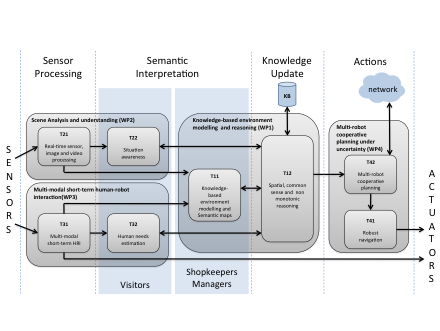
\includegraphics[height=10cm]{ArchitectureCoachesDF}
\caption{Architecture and data flow }
\label{Fig-1}
\end{center}
\end{figure}

\section{Use Cases}

The use cases are grouped in four scenarios that are described in the following sections.

\subsection{Scenario 1: Advertising and informing with simple interaction} 

\subsubsection*{Use Case 1.1: simple interaction and advertising} 

The use case adopted consists of a smart advertisement mission. The robots receive point of interests and plan to visit these points and announce the appropriate advertising according to the location. The points of interests should be focused on populated area and group detection. The robots should detect group of peoples, move toward this group, select a person to interact with and propose an appropriate advertisement according to the location and the interest expressed by the person. The robots should show a semantic map with appropriate shops with a path to head the shops. This use case illustrate the results developed in tasks T21, T22, T11, T12, T42, T41. 

The objective of this use case is to measure some performance indicators : percentage of good group detection for tasks T21 and T22 ; good expressiveness and message languages for T12 and map expressiveness T11 ; safe navigation and percentage of good advertisements according to the location. 

\subsubsection*{Use Case 1.2: Informing and guiding}

This use case consists in increasing the complexity of Scenario 1, by introducing the escorting and guiding services. The robot should guide the person to the destination, bu minting a permanent interaction during the escort or the guide. The customers should follow the robot to destination and the robot should adapt their behavior to the customers moving and behaviors.  The robots should be able to understand the abandon of the customers. This aspect allows us to assess the performance of  tasks T31 of estimating the need of the human. The human can also express their need via the multi-modal interface (Task T32).

The objective of this use case is to measure the same performance indicators as in scenario 1 but also the performance of tasks T31, T32 on the percentage of good need estimation. 

\subsection {Scenario 2: cooperation between robots}
The objective of this scenario is to extend Scenario 1 to a multi-robot system. In this scenario, we develop a use case to show the ability of robots to cooperate and to share tasks. 

\subsubsection*{Use Case 2.1: guiding many people with many robots in the same building}
In this use case, we extend  scenario 2 to different persons to guide or escort to different destinations. The robots should, in a decentralized way, share tasks (person or group to guide) and develop a coordinated strategy to assist all of them, to delegate a task if any unexpected event during the assistance and to inform the other robots about other persons to assist. The other aspect we present in this use case is the ability of robots to share space. 
The objective of this use case is to evaluate the performance of task 4.2.

\subsubsection*{Use Case 2.2: guiding many people from one building to another}
To this end,  we consider a use case  of guiding a person from one building to another where one robot guide the customer to the exit of building 1 and then  assist him to reach the building 2 where the second robot wait him and guides him to the destination. 
The objective of this scenario is to evaluate the tasks of WP4 and task T21. 

\subsection{Scenario 3: detecting abnormal events}

\subsubsection*{Use Case 3.1: Lost objects}
This use case consists of assessing the modules developed in WP2 in terms of perception. To this end, we consider a use case where external cameras detect object at a location (Task T21), the robot should evaluate if the  object is at a right or wrong location and generate an event (task T22) and the module of task T12 generates a task of visiting the location where the object is located. The robot moves towards the object and send a picture to an operator. 
The objective is mainly based on evaluating image processing task (T2.1).

\subsubsection*{Use Case 3.2: Abnormal activities}
This use case is mainly based on evaluating the human activities and assessing the situation. To this end, we consider the detection of some abnormal activities such as 
 the motionless of a customers, the robot moves toward the person and then interact with him to better assess his needs. The rest of interaction scenarii will be developed in use cases 5. Another aspect is to detect a person falling down to send a message for medical assistance if needed. We consider also the waving movement of a person to assess his hesitation and propose him a help;  

This use case allows us to evaluate the performance of tasks in WP2 and in WP3. 

\subsection{Scenario 4: Short-term interaction with customers}
The examples of this use case is to show different task assistances and interaction between the robot and the customers. The functionalities of tasks T3.1, T3.2, T1.2, T1.1, T4.1 and T4.2 will be presented and evaluated. 

\subsubsection*{Use Case 4.1 : Customer asks for help carrying his/her bag}
The robot is called by a manager (or by the customer himself) to assist
someone in carrying his/her bag. The robot must reach
the exit of the shop and approach the dedicated loading area. When
in position he looks for the customer and as soon as he establishes
contact, he asks the user to load the bag in the appropriate container.
Once loaded, the robot will ask the customer if he is in a hurry.
If the customer is in a hurry, the robot will proceed at a sustained
speed to the parking lot. In the other case, the robot will leisurely
proceed to the parking lot, proposing intermediate stops to shops
with interesting discounts.

The objective of this use case is to evaluate the performance of tasks T3.1, T3.2 and T4.2.
 
\subsubsection*{Use Case 4.2: Customer refuses first robot proposal, accepts specific one} Managers have told the robot that he needs to promote a special discount
for a movie. The robot is also aware, in his persistent KB, of the
existence of other secondary discounts. Since there are no people
moving around the robot starts waiting and scanning. As soon as it
sees a suitable user (at the right distance and the right speed),
the robot intercepts the customer and asks him/her if he would be interested
in the special discount for the movie. The user answers that s/he is not interested.
The robot then asks the user to slide his customer card in order to
propose the most appropriate available discount. After reading the
card, the robot finds out that the customer is a woman and that she
has made many purchases in the personal care department. 
So, the robot reasons that the special discount on the facial cream would be of interest
to her. After being informed of the discount, the customer reveals
to be interested and asks the robot for directions to reach the specific
shop. Since not many people are moving around, the robot can safely
guide the customer himself.
The objective of this use case is to evaluate the performance of tasks T3.1, T3.2, T4.2, T1.1 and T1.2.

\subsubsection*{Use Case 4.3 : Customer asks for directions in crowded environment} The robot has the objective to inform the customers of a certain few
available discounts. The shopping mall is very crowded and, for safety
considerations, the robot decides it should not move but rather wait
for users to approach. As soon as it detects a user, standing still at
the appropriate social distance, looking at him/her, the robot initiates
conversation and announces the available offers. The user is interested
and asks for directions. Since the robot cannot safely move, it shows
the desired path on his tablet and informs the user that 20m along
the corridor s/he will find another robot for more specific information,
if needed. The human thanks the robot and goes to the next one to
receive further directions.
The objective of this use case is to evaluate the performance of tasks T3.1, T3.2 and T4.1 and T4.2.

\subsection{Scenario 5: Short-term interaction with shopkeepers}
The examples of this use case is to show different task assistances and interaction between the robot and the shopkeepers. The functionalities of tasks T3.1, T3.2, T1.2, T1.1, T4.1 and T4.2 will be presented and evaluated. 


\subsubsection*{Use Case 5.1: Proposing ice creams to children} 
Manager from the local ice cream shop asks robot to inform children about
a special discount. The robot looks around for children. When it detects
one, it approaches him and informs him and his parents of the discount. The child
is passionate about having an ice cream; but before directing him
there, the robot asks for the parent's authorization. Once the parents
agree to allow the child to follow the robot, the robot will proceed
to the ice cream shop. 

The objective of this use case is to evaluate the performance of tasks T3.1, T3.2.

\subsubsection*{Use Case 5.2 : Shopkeepers ask for carrying bag of customers}
The robot receives messages from a shopkeepers to carry a bag from one location to another. The robot localizes the shop and navigates towards and then asks for the bags to transport and the customers to follow her. The robot should maintain a permanent interaction with the customer and uses the escort function to reach the destination. At the arrival the robot should ask the customers to take its bags and to confirm before leaving him. Without confirmation from the customer, the robot asks the customer to take bags and confirm. After three times, the robot send message to the shopkeeper and come back to the shop for keeping the bags or confirming.

The objective of this use case is to evaluate the performance of tasks T3.1, T3.2, T4.1 T4.2, T1.2 and T1.1.

\subsection {Demonstration}
We propose to use the robots in the Rives De l'Orne Mall of the Caen city, in the collaboration of the city's representative and the Rive de l'Orne manager
\newpage
\section{Test facilities: Collaboration with the Mall Rives de l'Orne}
The test facilities concerns the Mall Rives de l'Orne. � Rive de l�orne � is a new and modern mall at Caen city (France). It is composed of two face-to-face buildings separated by a large main square. At the first floor of the two buildings, there are many shops and restaurants. In the main square, there is a cinema. This space is surrounded by tramway stations and a train station. This mall is visited by more than 100,000 customers every year. In addition to that, several elderly people live in the new apartments at the other floors of the buildings. These people have their habit and there are frequent customers of the mall \ref{mall}. Two meetings have been organized ($23^{th}$ October and $12^{th}$ December 2014)to define the equipments to install in terms of cameras and sensors (RFID) to send some information to robots about shops, the planning of the robot deployment in the mall and some local dissemination actions. A visit of all partners have been organized during the kickoff meeting. 

\begin{figure}[htbp]
\begin{center}
\includegraphics[height=5cm]{InsideRivedelOrne}
\caption{Inside the mall}
\label{mall}
\end{center}
\end{figure}

\begin{figure}[htbp]
\begin{center}
\includegraphics[height=5cm]{MapsRorne}
\caption{The map}
\label{default}
\end{center}
\end{figure}



\section{Demonstrations}
\label{sec:demo}

The scenario where the COACHES robots and systems will be deployed, demonstrated, and validated is provided by the mall ``Rives de l'Orne''\footnote{\url{http://www.rivesdelorne.com}}, located in the city of Caen, France  (see Fig. \ref{fig:outsidemall}).

\begin{figure}[!t]
\begin{center}
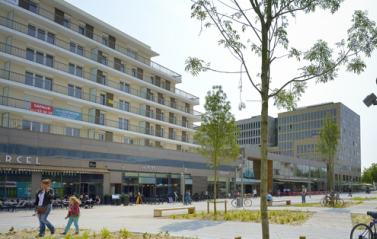
\includegraphics[width=0.55\linewidth]{fig/outsiderivesdelorne}
\caption{The mall Rives de l'Orne.}
\label{fig:outsidemall}
\end{center}
\end{figure}

\begin{figure}[htbp]
\begin{center}
\includegraphics[height=5cm]{fig/MapsRorne}
\caption{The map}
\label{fig:map}
\end{center}
\end{figure}

\begin{figure}[htbp]
\begin{center}
\includegraphics[height=6cm]{fig/InsideRivedelOrne}
\caption{Inside the mall}
\label{fig:insidemall}
\end{center}
\end{figure}

The test facility is a new and modern mall composed of two face-to-face buildings separated by a large main square. Figure \ref{fig:map} shows a plan of the mall.
At the first floor of the two buildings, there are many shops and restaurants (as shown in Figure \ref{fig:insidemall}). In the main square, there is a cinema. This space is surrounded by tramway stations and a train station. This mall is visited by more than 100,000 customers every year. In addition to that, several elderly people live in the new apartments at the other floors of the buildings. These people have their habit and there are frequent customers of the mall. 

Two meetings have been organized ($23^{th}$ October and $12^{th}$ December 2014) to define the equipments to install in terms of sensors.

Cameras and other sensors are in charge of sending information to the COACHES robots about the environment.
%\begin{itemize}
%\item the shops;
%\item the planning of the robot deployment in the mall;
%\item the scheduled dissemination actions.
%\end{itemize}
Moreover, Radio-Frequency IDentification (RFID) tags and receivers could be used to identify shops and possibly key people for the application.

The shopping mall is a perfect environment to test and validate the use cases described in the previous section. Some of them will be thus fully implemented and tested with real customers of the shopping mall, within the course of the project.



\subsection{Testing the use cases}

The use cases described above will be tested in the shopping mall of Caen with the following procedure.
\begin{enumerate}
\item Description to shop keepers and managers to collect feedback and apply modifications or provide more details.
\item Test with real users using a mock-up implementation where the robot is driven by a user operator.
\item Implementation and test of the fully autonomous behavior in an incremental way, by allowing at intermediate phases the use of non-fully autonomous components.
\item Final test of the fully autonomous behaviors with real users.
\end{enumerate}








\section{Use cases for short-term interaction and safe navigation}
\label{sec:usecase_sapienza}

As described in the previous sections,
COACHES project envisages the implementation of a set of use cases
to show the feasibility of the approach and to assess the effectiveness
of the proposed solutions with actual users.

Four use cases that are mainly related with short-term human-robot interaction and safe navigation are described in the following. These use cases correspond to the ones in Scenarios 4 and 5 described above\footnote{Use Case 5.2 is not reported in details here since it is similar to Use Case 4.1.}.
Other use cases illustrated before can be considered as preliminary tests to the ones described in this section. Therefore, we report here in details only the most complex ones.

For each use case, the following data are provided:
\begin{itemize}
\item A brief textual description;
\item One (or more) sequence diagrams;
\item An optimistic sequence of actions.
\end{itemize}

Furthermore, a detailed overview of the preconditions and post-conditions for each action executed by the robots is given in Section \ref{sec:robot_actions}.


\subsection{Use Case 4.1: Customer asks for help carrying his/her bag}

The objective of this use case is to highlight the social awareness
of the robot in the completion of a given task. There are many ways
to carry a bag for a customer, but only a few might be socially acceptable
at a given moment. To perform well, the robot asks the customer about her/his priorities.

\subsubsection{Use case description}

The robot is called by a shop manager (or by a customer) to help
in carrying bags. Bag loading operations take place in dedicated areas,
located at the exit of the shops.
The robot has to
\begin{enumerate}
\item Reach the exit of the shop;
\item Approach the dedicated bag loading area.
\end{enumerate}

\noindent When in position, the robot waits for the customer to establish
a contact.
Once the customer has established a contact, the robot asks the user
to load the bag in the bin carried by the robot.
Once the bag is loaded, the robot asks the customer if she/he is in a hurry.
If the customer is in a hurry, the robot
\begin{enumerate}
\item sets its speed to a high value;
\item proceeds to the mall parking lot.
\end{enumerate}

\noindent In the other case, the robot
\begin{enumerate}
\item sets its speed to a low value;
\item proceeds to the mall parking lot, proposing intermediate stops to shops
with possible interesting offers for the customer.
\end{enumerate}

In any case the robot modulates its speed taking into account the number of detected people, to minimize the risk of collision.

\subsubsection{Sequence diagram}

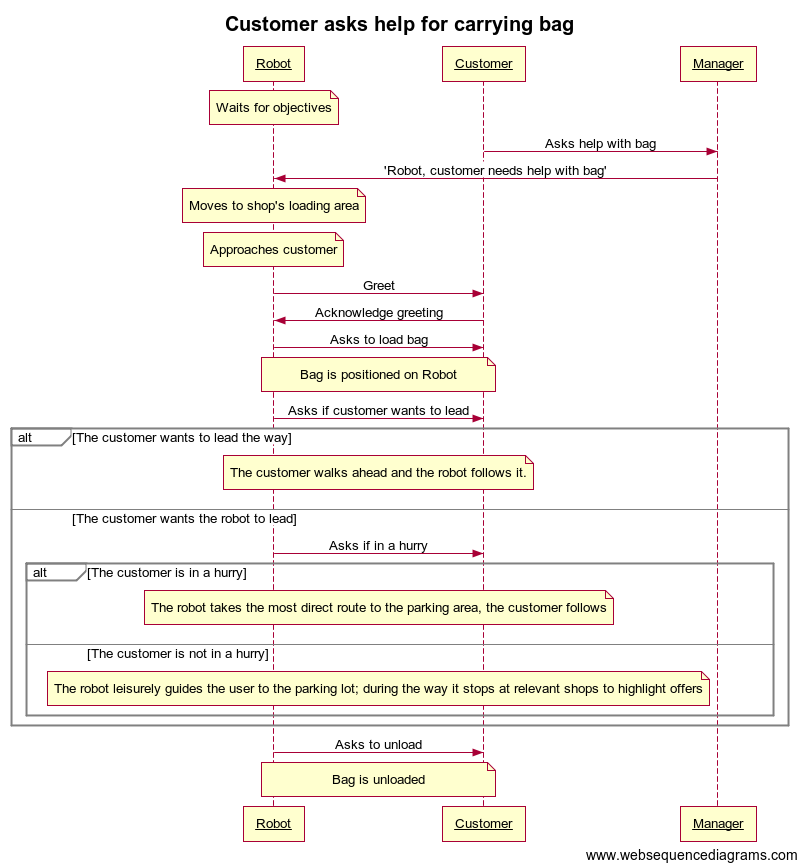
\includegraphics[width=0.85\textwidth]{bagUseCase}


\subsubsection{Optimistic robot action sequence}
\begin{enumerate}
\item Go to shop's loading area
\item Approach customer
\item Start conversation
\item Ask to load bag
\item Ask if customer wants to lead
\item Follow customer
\item Ask To Unload
\item End conversation
\end{enumerate}

\subsection{Use Case 4.2: Customer refuses first robot proposal and accepts a different one}

This use case highlights how the robot is capable of
recovering from a failure by exploiting automatic reasoning.
Since the customer refuses the first offer proposed by the robot, instead of randomly proposing a new offer to her/him, the robot tries to understand the user's preferences.

Moreover, in this use case, the proactive nature of the robot's behavior (when allowed by security concerns) is also underlined: when no people are
moving around, the robot can decide to approach itself a customer.

\subsubsection{Use case description}

The sales manager of a cinema inside the mall needs to promote a special discount
for a movie. The discount is loaded by the manager into the 
knowledge base (KB) of the robot, that contains the list of all the active commercial offers.
The robot is also aware, in his persistent KB, of the
existence of other secondary discounts.

Since there are no people moving around the robot, it starts
waiting for customers by monitoring the scene. As soon as the robot
sees a potential user (moving at the right distance and at the right speed),
the robot intercepts the customer and it asks her/him if she/he is interested
in the special discount for the movie.

The user answers that she/he is not interested.
Then, the robot asks the user to slide her/his personal customer card in order to
obtain a different available discount, in accordance to the user's previous purchases.

After the card data has been read, the robot finds out that the customer is a woman and that she
has made many purchases in the personal care department. 
Thus, the robot, by analysing the list of all the active commercial offers,
infers that the special discount about a facial cream could be of interest
to her.

Once informed of the discount, the customer reveals
that she is interested in it and she asks the robot for directions to reach the specific
shop. The robot safely guides the customer to the shop.

\newpage

\subsubsection{Sequence diagram}

\begin{figure}[!h]

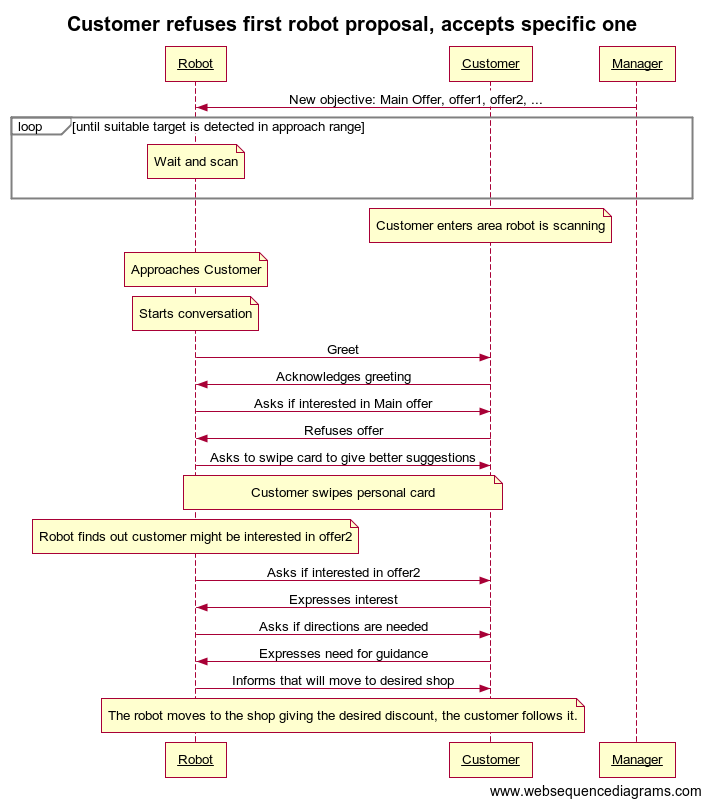
\includegraphics[width=0.75\textwidth]{offerReasoning}

\end{figure}



\subsubsection{Optimistic robot action sequence}
\begin{enumerate}
\item Approach customer
\item Start conversation
\item Propose main offer (in this use case we assume this fails)
\item Ask for the customer to identify himself by swiping the card
\item Find appropriate offer for user
\item Propose new offer to user
\item Ask customer to follow
\item Go to appropriate shop
\item Inform customer destination has been reached
\item End conversation
\end{enumerate}


\subsection{Use Case 4.3: Customer asks for directions in a crowded environment}

The goal of this use case is to remark that the robot must always be
aware of safety. The robot is not allowed to behave hazardously
in presence of humans.

\subsubsection{Use case description}

The robot has the objective to inform customers of available discounts.
The shopping mall is very crowded and, for safety
reasons, the robot decides that it should not move around, but
that is more convenient to wait
for users to approach it.

As soon as it detects a user, standing still at
the appropriate social distance and looking at her/him, the robot initiates
a conversation and it announces the available offers.

The user is interested in a listed offer
and she/he asks for directions to reach the shop offering a discount.
Since the robot cannot safely move due to the crowded environment, it
\begin{enumerate}
\item shows the user the desired path on its tablet;
\item informs the user that 20 meters away along the corridor she/he will find another robot,
that can provide more specific information, if needed.
\end{enumerate}

\noindent The human thanks the robot and proceeding to the next one in order to
receive further directions.

\subsubsection{Sequence diagrams}

\begin{figure}[!h]
\fbox{\begin{minipage}[t]{0.48\columnwidth}%
\begin{center}
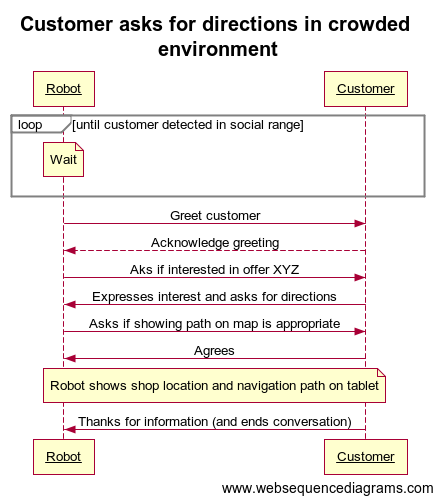
\includegraphics[width=1\textwidth]{crowdedCaseA}
\par\end{center}

\begin{center}
\textit{Robot shows path on map}
\par\end{center}%
\end{minipage}}\hfill{}%
\fbox{\begin{minipage}[t]{0.48\columnwidth}%
\begin{center}
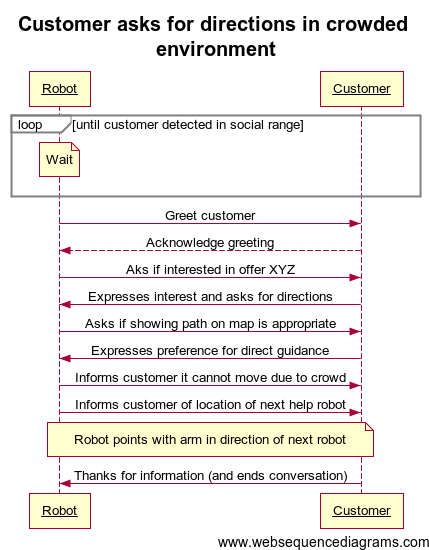
\includegraphics[width=1\columnwidth]{crowdedCaseB}
\par\end{center}

\begin{center}
\textit{Robot shows where next helper is}
\par\end{center}%
\end{minipage}}

%\protect\caption{Customer asks for directions in crowded environment}


\end{figure}



\subsubsection{Optimistic robot action sequence}

\textit{A human approaches the robot}
\begin{enumerate}
\item Start conversation
\item Ask if interested in offer XYZ
\item Ask if showing path on map is appropriate
\item Show path to shop on tablet
\item End conversation
\end{enumerate}


\subsection{Use Case 5.1: Proposing an ice cream to a child}

This use case serves to demonstrate the common sense reasoning capability
of the robot. Since it is not socially acceptable for the robot to guide
a child to a location without her/his parents permission, the robot
asks for the parent's permission before completing the task.

\subsubsection{Use case description}

The manager of an ice cream shop asks the robot to inform children about
a special offer. The robot looks around for children. When it detects
a child, the robot approaches her/him and it informs her/him
about the special offer. The child is passionate about having an ice cream, 
but, before guiding her/him to the ice cream shop, the robot
\begin{enumerate}
\item asks for the parent's authorization,
\item waits for the positive parent's reply.
\end{enumerate}

\noindent Once the parent agrees to allow the child to follow the robot, it proceeds
to the ice cream shop.

\subsubsection{Sequence diagrams}

\begin{figure}[!h]
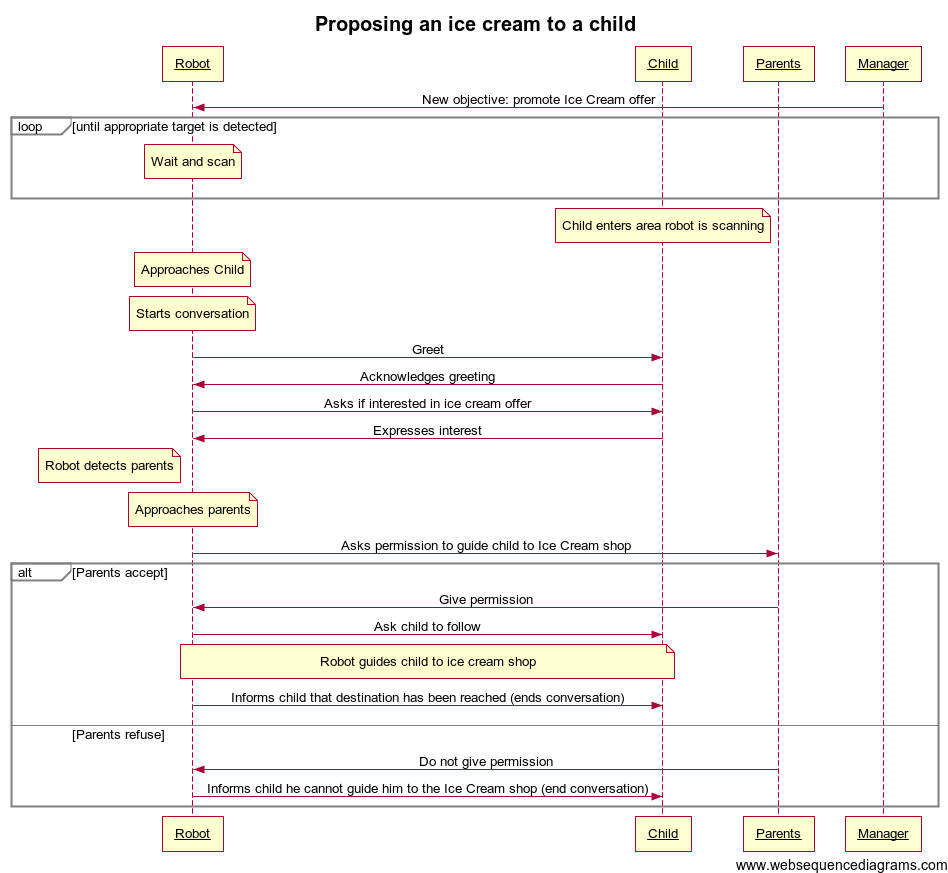
\includegraphics[width=0.85\textwidth]{iceCreamA}
\protect\caption{Option A: Parents are near the child.}
\end{figure}


\begin{figure}[!h]
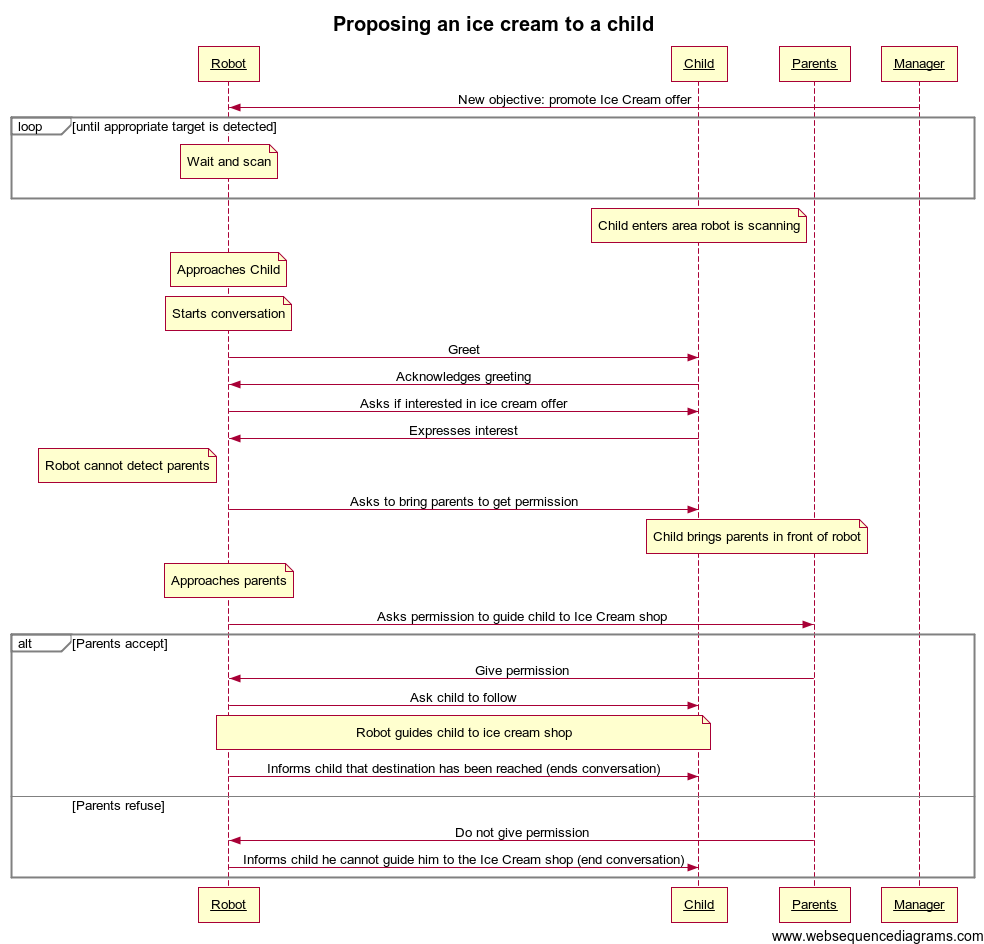
\includegraphics[width=0.85\textwidth]{iceCreamB}
\protect\caption{Option B - Parents are not near the child.}
\end{figure}



\subsubsection{Optimistic robot action sequence}
\begin{enumerate}
\item Approach child
\item Start conversation
\item Describe ice cream offer
\item Ask parents for permission
\item Ask child to follow
\item Go to IceCreamShop
\item Inform customer destination has been reached
\item End conversation
\end{enumerate}




\subsection{Robot actions}
\label{sec:robot_actions}

In this section, the actions that the robot has to perform in order to
accomplish its tasks are described.
For each action, the preconditions and the post conditions that must hold are
listed. 


\subparagraph{Approach Human(Human)}

:

\textit{Prec}: The human has been detected by sensors and is reachable.

\textit{Post}: The robot positions itself at a social distance from
the user, possibly in plain view and facing the human.

\textit{Description}: This action usually precedes starting a conversation


\subparagraph{AskHumanIfInHurry(Human)}

:

\textit{Prec}: The robot is carrying something belonging to the human,
the human asked to robot to lead

\textit{Post}: The fact that the human is in a hurry or not, is added
to the knowledge base.

\textit{Description}: This question is asked to understand if the
robot should move directly to the parking area or can show a few offers
during the way


\subparagraph{AskHumanToDeload(Human)}

:

\textit{Prec}: The robot is carrying something belonging to the human

\textit{Post}: The human's object is removed from the robot

\textit{Description}: If the human refuses to remove the object, a
manager should be notified.


\subparagraph{AskHumanToLoad(Human)}

:

\textit{Prec}: The robot is in conversation with the human

\textit{Post}: The human's bag is on top of the robot

\textit{Description}:


\subparagraph{AskHumanWhoLeads(Human)}

:

\textit{Prec}: The robot is carrying something belonging to the human

\textit{Post}: The fact that the human wants to lead, or the contrary,
is added to the knowledge base.

\textit{Description}: This question is asked to understand if the
robot must lead or follow the human

 


\subparagraph{End Conversation(Human)}

:

\textit{Prec}: Human and robot are engaged in conversation.

\textit{Post}: Human and robot are no longer engaged in conversation.

\textit{Description}: The robot follows a social protocol to end the
conversation (es: ``See you next time!'')


\subparagraph{Engage Conversation(Human)}

:

\textit{Prec}: Robot is in social range with human. Human can see
robot, robot is facing human.

\textit{Post}: Human and robot are engaged in conversation.

\textit{Description}: The robot follows a social protocol to start
the conversation (``Hello human'') and make sure the human is interested


\subparagraph{Goto(Destination)}

:

\textit{Prec}: There is a path to the destination.

\textit{Post}: The robot is now at(Destination)

\textit{Description}: The robot navigate in a socially aware way to
the desired location.

\section{Conclusions}
\label{sec:conclu}

In this paper, we have described the main concepts of the \coaches project and in particular its Artificial Intelligence and Robotics components and their integration. 
More specifically, we have described a framework for integrating knowledge representation and reasoning, MDP planning and PNP execution, allowing a feedback from execution to reasoning in order to update and improve the current model of the world. 
Implementation and preliminary tests of such an integration have been performed to assess the suitability of the proposed architecture.
%While most of the project will be developed and experimented in the next years, the design and the preliminary tests reported in this paper show the feasibility and the effectiveness of the proposed approach.

Many interesting results are expected from the \coaches project, since the environment and the challenges considered here are very ambitious. 
Among the several performance evaluation procedures, we aim at including extensive user studies that will be used to validate the effective development of intelligent social robots performing complex tasks in public populated areas. 

We believe that deploying robots in public spaces populated by non-expert users is a fundamental process for the actual design, development and validation of integrated research in Artificial Intelligence and Robotics. Consequently, we envision many significant contributions to this research area from the \coaches project.








